\documentclass[12pt,a4paper]{article}

% ── Packages ──────────────────────────────────────────────────────────────────
\usepackage[utf8]{inputenc}
\usepackage[T1]{fontenc}
\usepackage[english]{babel}
\usepackage{geometry}
\geometry{a4paper, margin=2.5cm}

\usepackage{amsmath}
\usepackage{amssymb}
\usepackage{graphicx}
\usepackage{float}
\usepackage{booktabs}
\usepackage{array}
\usepackage{multirow}
\usepackage{xcolor}
\usepackage{hyperref}
\usepackage{natbib}
\usepackage{caption}
\usepackage{subcaption}
\usepackage{setspace}
\usepackage{fancyhdr}
\usepackage{abstract}
\usepackage{titlesec}
\usepackage{parskip}
\usepackage[activate=false]{microtype}
\usepackage{url}
\usepackage{siunitx}

% ── Colours ───────────────────────────────────────────────────────────────────
\definecolor{ssp245}{RGB}{41,128,185}
\definecolor{ssp585}{RGB}{192,57,43}
\definecolor{era5col}{RGB}{39,174,96}
\definecolor{headcol}{RGB}{44,62,80}

% ── Hyperref setup ────────────────────────────────────────────────────────────
\hypersetup{
  colorlinks = true,
  linkcolor  = headcol,
  citecolor  = headcol,
  urlcolor   = ssp245,
  pdftitle   = {Extreme Heat and Drought Events in the Carpathian Basin},
  pdfauthor  = {Earth2Research Project},
}

% ── Page style ────────────────────────────────────────────────────────────────
\pagestyle{fancy}
\fancyhf{}
\rhead{\small Carpathian Basin Extreme Climate Events}
\lhead{\small Earth2Studio | ARCO-ERA5 | CMIP6}
\cfoot{\thepage}
\renewcommand{\headrulewidth}{0.4pt}

% ── Title formatting ──────────────────────────────────────────────────────────
\titleformat{\section}{\large\bfseries\color{headcol}}{}{0em}{}[\titlerule]
\titleformat{\subsection}{\normalsize\bfseries\color{headcol}}{}{0em}{}

% ── Line spacing ─────────────────────────────────────────────────────────────
\onehalfspacing

% ── Caption setup ─────────────────────────────────────────────────────────────
\captionsetup{font=small, labelfont=bf, margin=10pt}

% ─────────────────────────────────────────────────────────────────────────────
\begin{document}

% ── Title block ───────────────────────────────────────────────────────────────
\begin{titlepage}
  \centering
  \vspace*{1.5cm}

  {\LARGE\bfseries\color{headcol}
    Extreme Heat Dome and Drought Events\\[0.4em]
    in the Carpathian Basin:\\[0.4em]
    Historical Validation and Climate Projections\\[0.4em]
    to 2075 Using NVIDIA Earth2Studio
  \par}

  \vspace{1.5cm}

  {\large Earth2Research Project\par}
  \vspace{0.5cm}
  {\normalsize
    Carpathian Basin Climate Analysis Group\\
    Pápa, Veszprém, Hungary
  \par}

  \vspace{1cm}
  {\normalsize \today\par}

  \vspace{2cm}

  \begin{abstract}
    \noindent
    We present an analysis of extreme heat dome and drought events in the
    Carpathian Basin using the NVIDIA Earth2Studio framework with ARCO-ERA5
    reanalysis data and CMIP6 climate projections. Three historical extreme
    events are examined: the 2003 European Heatwave, the 2012 Pannonian
    Drought, and the 2021 Balkan Heat Dome. For each event we extract
    2\,m temperature and 500\,hPa geopotential height fields and evaluate
    48-hour forecast skill using three baseline methods — Persistence,
    Climatology, and Linear Trend Extrapolation — against ERA5 ground truth.
    We find that no single forecast method dominates across all event types:
    rapid-onset heat domes are best captured by linear trend extrapolation
    (ACC up to 0.95), while slow-building drought events are better described
    by climatological baselines. The 2021 heat dome emerges as the most
    anomalous event (peak T2m = 39.6\,°C), causing a catastrophic failure of
    climatological forecasts (bias = --9.69\,°C). Future projections using
    the MPI-ESM1-2-LR CMIP6 model under SSP2-4.5 and SSP5-8.5 scenarios
    indicate regional July mean temperatures will exceed the 1995--2010
    baseline by +4.5\,°C (SSP2-4.5) and +6.0\,°C (SSP5-8.5) by the
    2065--2074 decade, with the southern Carpathian Basin warming fastest.
    Both scenarios breach the Paris Agreement 2\,°C threshold before 2035
    for this region, highlighting the urgency of emission reductions.
    All data, code, and figures are openly available.
  \end{abstract}

  \vspace{1cm}

  \noindent\textbf{Keywords:} heat dome; drought; Carpathian Basin; Hungary;
  ERA5 reanalysis; CMIP6; Earth2Studio; climate projection; extreme events;
  forecast skill

\end{titlepage}

% ─────────────────────────────────────────────────────────────────────────────
\section{Introduction}
\label{sec:intro}
% ─────────────────────────────────────────────────────────────────────────────

The Carpathian Basin, encompassing Hungary and surrounding lowland regions,
is among the most climatically vulnerable areas in Europe. Situated at the
intersection of continental, Mediterranean, and Atlantic weather regimes,
the basin experiences both severe summer heat events and multi-season
droughts with increasing frequency \citep{ipcc2021}. The 2003 European
Heatwave, the 2012 Pannonian Drought, and the 2021 Balkan Heat Dome each
caused significant agricultural losses, public health crises, and
infrastructure stress across the region.

Artificial intelligence-based weather and climate modelling has advanced
rapidly in recent years. Tools such as Pangu-Weather \citep{bi2023accurate},
FourCastNet \citep{pathak2022fourcastnet}, and GraphCast
\citep{lam2023graphcast} have demonstrated forecast skill comparable to or
exceeding traditional numerical weather prediction (NWP) for certain
variables and lead times. The NVIDIA Earth2Studio framework
\citep{earth2studio2024} provides a unified, open-source pipeline for
accessing these models alongside high-quality reanalysis and climate
projection datasets.

This study makes three contributions. First, we demonstrate how
Earth2Studio can be used to extract, analyse, and visualise ERA5 reanalysis
data for regional extreme event studies at low computational cost, using
only a consumer-grade GPU (NVIDIA GeForce RTX\,4070, 12\,GB VRAM).
Second, we evaluate 48-hour forecast skill for temperature fields across
three historically significant extreme events using standard meteorological
baseline methods, providing a quantitative assessment of predictability
characteristics for each event type. Third, we provide decade-by-decade
climate projections for the Carpathian Basin through 2075 using CMIP6
output under two emission scenarios, contextualised against Paris Agreement
thresholds.

% ─────────────────────────────────────────────────────────────────────────────
\section{Data and Methods}
\label{sec:methods}
% ─────────────────────────────────────────────────────────────────────────────

\subsection{Study Region}

The study domain covers the Carpathian Basin, defined here as the
rectangular region 44.0--49.5\,°N, 14.0--23.5\,°E. This encompasses
Hungary in its entirety, together with adjacent lowland areas of Austria,
Slovakia, Romania, Serbia, and Croatia. The basin is characterised by
a continental climate with hot summers (July mean T2m $\approx$ 19\,°C
in the ERA5 climatology) and a marked north--south gradient in temperature
and precipitation during summer months.

\subsection{ERA5 Reanalysis Data}

Atmospheric reanalysis data were obtained from the ARCO-ERA5 dataset
\citep{carver2023arco}, accessed via the Earth2Studio \texttt{ARCO} data
source interface. ARCO-ERA5 provides the complete ERA5 reanalysis on a
0.25\,° × 0.25\,° global grid at 6-hourly temporal resolution, hosted on
Google Cloud Storage and publicly accessible without registration. Two
primary variables were extracted:

\begin{itemize}
  \item \textbf{T2m}: 2\,m air temperature (K, converted to °C)
  \item \textbf{Z500}: 500\,hPa geopotential (m\textsuperscript{2}\,s\textsuperscript{--2},
        converted to geopotential height in metres by dividing by
        $g = 9.80665$\,m\,s\textsuperscript{--2})
\end{itemize}

All ERA5 data were retrieved at 12:00\,UTC (12\,Z) to capture peak
daytime temperatures.

\subsection{CMIP6 Climate Projections}

Future climate projections were obtained from the Coupled Model
Intercomparison Project Phase 6 (CMIP6) archive \citep{eyring2016overview}
via the Earth2Studio \texttt{CMIP6} data source, which wraps the
\texttt{intake-esgf} catalogue interface. We used the MPI-ESM1-2-LR model
\citep{mpi2019}, ensemble member r1i1p1f1, monthly atmospheric output
(CMOR table \texttt{Amon}), under two Shared Socioeconomic Pathway (SSP)
scenarios:

\begin{itemize}
  \item \textbf{SSP2-4.5}: ``Middle of the road'' moderate emission
        scenario, reaching approximately 4.5\,W\,m\textsuperscript{--2}
        radiative forcing by 2100.
  \item \textbf{SSP5-8.5}: ``Fossil-fuelled development'' high emission
        scenario, reaching approximately 8.5\,W\,m\textsuperscript{--2}
        radiative forcing by 2100.
\end{itemize}

A historical baseline was established using the \texttt{historical}
experiment for the period 1995--2010. July monthly mean T2m was used
throughout as a representative peak-summer variable.

\subsection{Historical Events}

Three events were selected to represent the range of extreme summer
conditions affecting the Carpathian Basin (Table~\ref{tab:events}).

\begin{table}[H]
  \centering
  \caption{Historical extreme events analysed in this study.}
  \label{tab:events}
  \begin{tabular}{llll}
    \toprule
    \textbf{Event} & \textbf{Peak Date} & \textbf{Type} & \textbf{Peak T2m (°C)} \\
    \midrule
    2003 European Heatwave  & 12 Aug 2003, 12\,Z & Heat dome & 39.4 \\
    2012 Pannonian Drought  & 20 Jul 2012, 12\,Z & Drought   & 38.4 \\
    2021 Balkan Heat Dome   & 24 Jun 2021, 12\,Z & Heat dome & 39.6 \\
    \bottomrule
  \end{tabular}
\end{table}

\subsection{Forecast Validation Methodology}

For each event, ERA5 fields at 48\,h prior to the peak were used as
initial conditions, and three baseline forecast methods were applied:

\paragraph{Persistence.}
The T2m field at $t_0 - 48$\,h is used unchanged as the forecast for
time $t_0$. This is the standard meteorological baseline: if a forecast
cannot beat persistence, it has no skill.

\paragraph{Climatology.}
The mean T2m field for the same calendar day across the 1991--2010
reference period (20 years, ERA5) is used as the forecast. A climatological
forecast captures the expected seasonal state but not synoptic anomalies.

\paragraph{Linear Trend Extrapolation.}
A pixel-wise ordinary least squares regression is fitted to the five
daily ERA5 T2m fields spanning $t_0 - 5$\,days to $t_0 - 1$\,day, and
extrapolated to $t_0$. This captures the direction of the temperature
tendency leading into the event.

Three skill scores are computed for each method and event
(Equations~\ref{eq:rmse}--\ref{eq:acc}):

\begin{align}
  \text{RMSE} &= \sqrt{\frac{1}{N}\sum_{i=1}^{N}(F_i - O_i)^2}
  \label{eq:rmse} \\[6pt]
  \text{Bias} &= \frac{1}{N}\sum_{i=1}^{N}(F_i - O_i)
  \label{eq:bias} \\[6pt]
  \text{ACC}  &= \frac{\sum_{i=1}^{N} F'_i O'_i}
                      {\sqrt{\sum_{i=1}^{N} F'^2_i \sum_{i=1}^{N} O'^2_i}}
  \label{eq:acc}
\end{align}

where $F_i$ and $O_i$ are forecast and observed (ERA5) T2m values at
grid point $i$, $F'_i = F_i - \bar{F}$ and $O'_i = O_i - \bar{O}$ are
spatial anomalies, and $N$ is the number of grid points in the domain.
An ACC $\geq 0.6$ is the conventional threshold for a ``skillful''
forecast \citep{wilks2011}.

\subsection{Computational Environment}

All analysis was performed on a desktop workstation equipped with an
Intel Core i5 CPU, 32\,GB RAM, and an NVIDIA GeForce RTX\,4070 GPU
(12\,GB VRAM) running Windows 11. The software environment used
Python 3.12 with Conda package management, Earth2Studio (latest),
PyTorch 2.x with CUDA 12.4, xarray, Cartopy, and Matplotlib.

% ─────────────────────────────────────────────────────────────────────────────
\section{Results}
\label{sec:results}
% ─────────────────────────────────────────────────────────────────────────────

\subsection{Historical Event Characterisation}

Figure~\ref{fig:comparison} shows the peak-day 2\,m temperature fields
for all three events on a common colour scale. The 2021 Balkan Heat Dome
(peak T2m = 39.6\,°C) covers the largest area of extreme heat and
exhibits the most spatially uniform warm anomaly across the basin,
consistent with a strong, persistent high-pressure ridge. The 2003
heatwave (39.4\,°C) shows a stronger spatial gradient, with the western
portions of the domain remaining cooler. The 2012 drought peak (38.4\,°C)
is most intense in the south-eastern sector.

\begin{figure}[H]
  \centering
  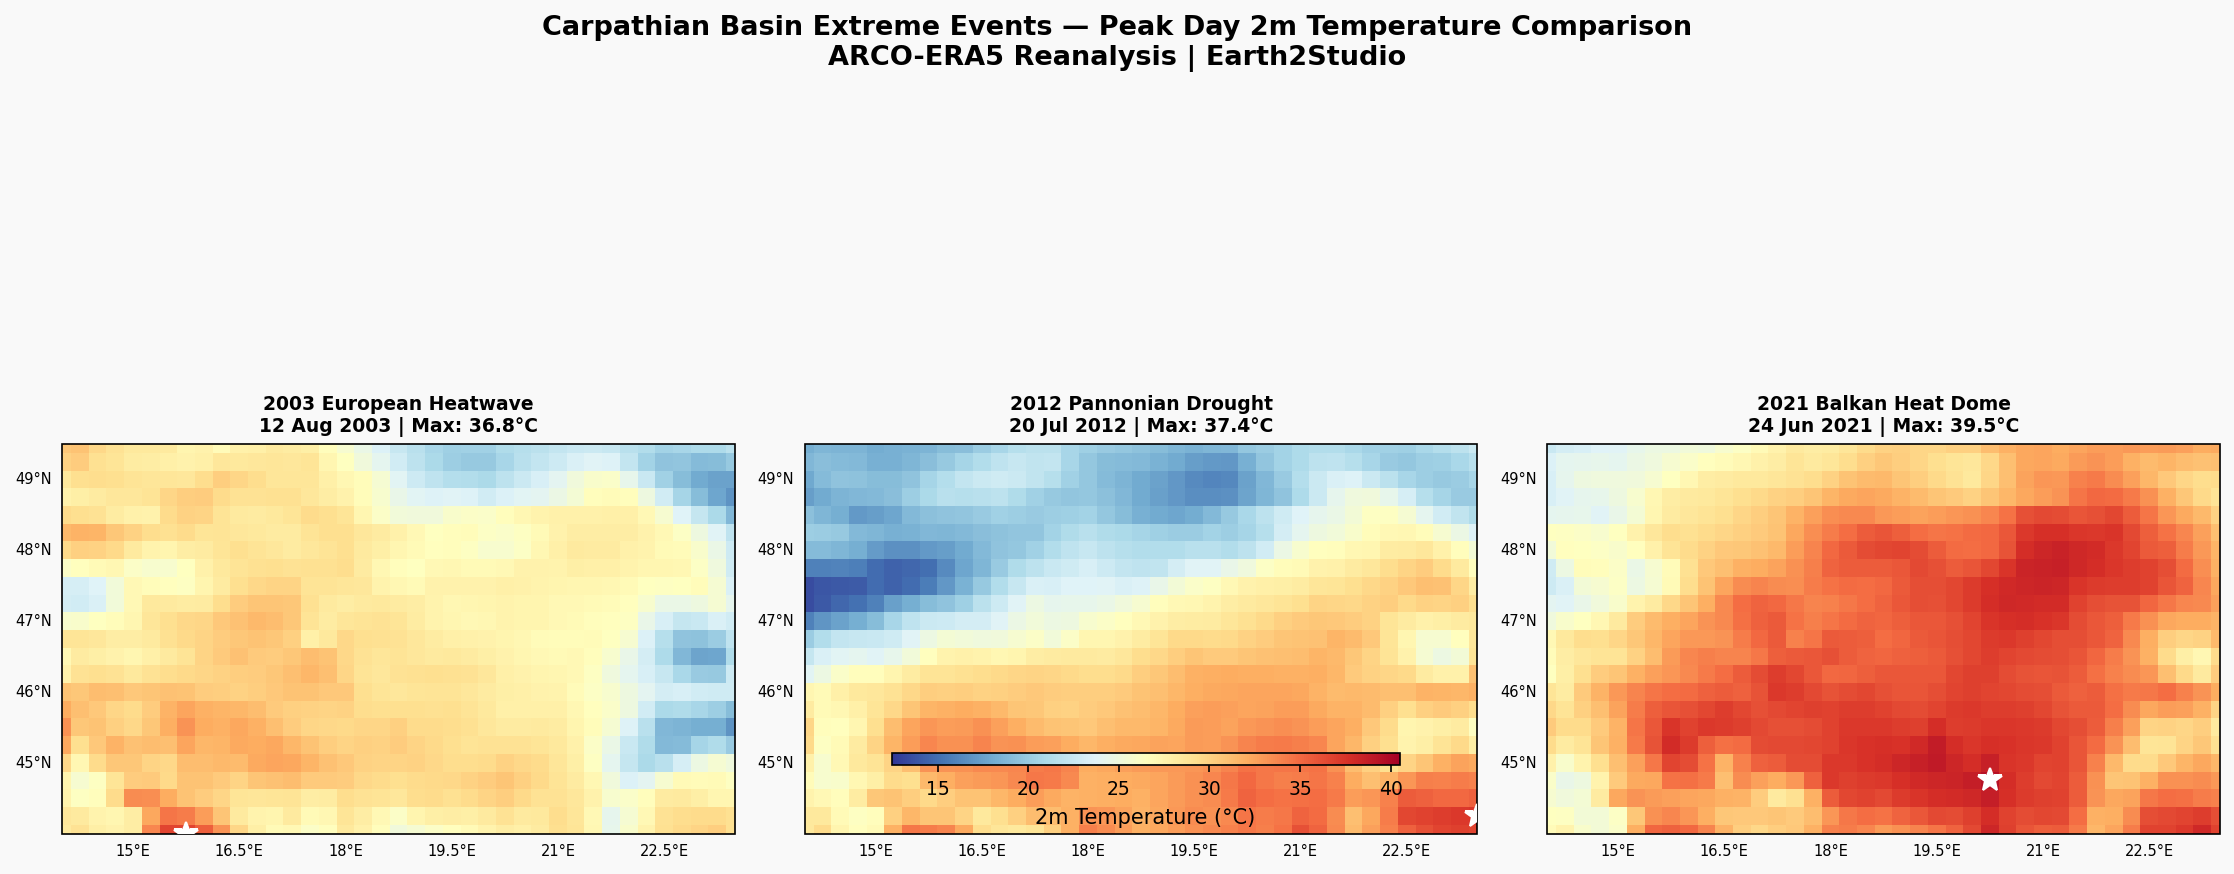
\includegraphics[width=\textwidth]{figures/historical/02_three_event_comparison.png}
  \caption{Peak-day 2\,m temperature (T2m) for the three historical
    extreme events over the Carpathian Basin. ERA5 reanalysis at 12\,Z,
    accessed via ARCO-ERA5 through Earth2Studio. The white star marks
    the grid-point maximum in each panel.}
  \label{fig:comparison}
\end{figure}

Figure~\ref{fig:heatwave2003} shows the dual-panel analysis for the
2003 event, displaying T2m alongside the 500\,hPa geopotential height
field (Z500). The Z500 ridge exceeding 5880\,m in the western sector
is a diagnostic signature of a heat dome: an anomalously strong
upper-level anticyclone that suppresses convection and traps heat near
the surface.

\begin{figure}[H]
  \centering
  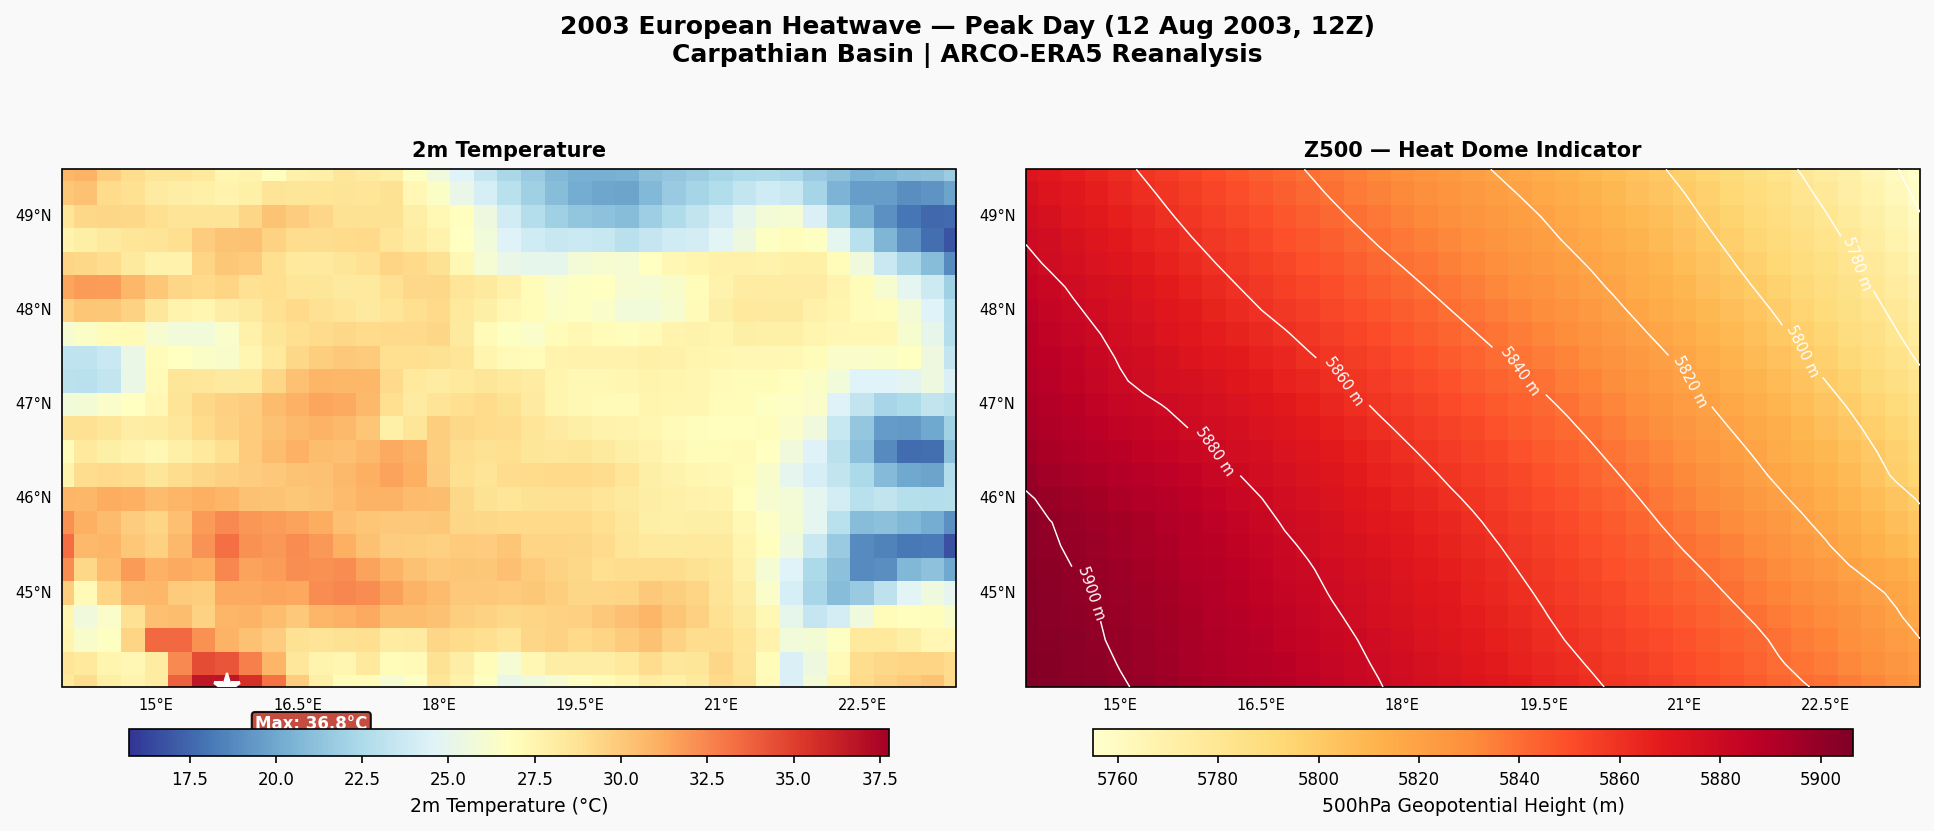
\includegraphics[width=0.95\textwidth]{figures/historical/02_heatwave_2003_peak_map.png}
  \caption{2003 European Heatwave peak day (12 Aug 2003, 12\,Z).
    Left: 2\,m temperature (T2m). Right: 500\,hPa geopotential height
    (Z500), a diagnostic indicator of heat dome structure. Contour lines
    at 25\,m intervals. ERA5 reanalysis via Earth2Studio ARCO source.}
  \label{fig:heatwave2003}
\end{figure}

\begin{figure}[H]
  \centering
  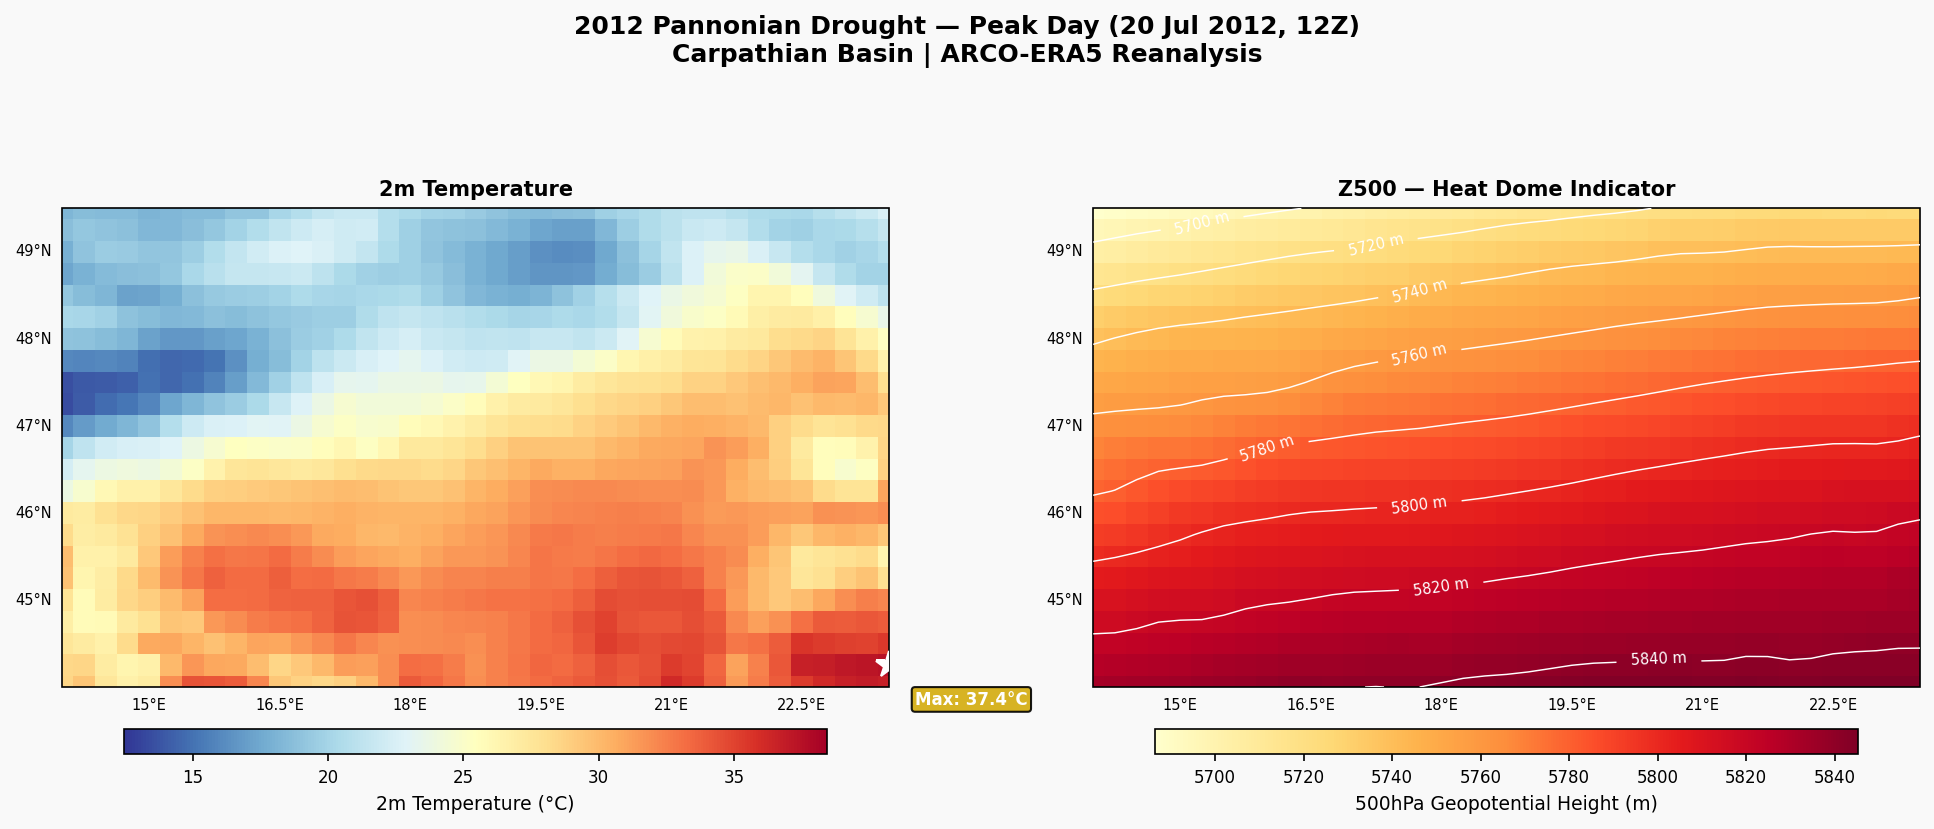
\includegraphics[width=0.95\textwidth]{figures/historical/02_drought_2012_peak_map.png}
  \caption{2012 Pannonian Drought peak day (20 Jul 2012, 12\,Z).
    The Z500 ridge is displaced southward relative to 2003, consistent
    with a Pannonian heat low driving surface warming across the
    south-eastern basin.}
  \label{fig:drought2012}
\end{figure}

\subsection{Forecast Skill Assessment}

Table~\ref{tab:scores} and Figure~\ref{fig:skill} summarise the 48-hour
forecast skill scores for all three methods across the three events.

\begin{table}[H]
  \centering
  \caption{48-hour forecast skill scores for T2m over the Carpathian
    Basin. Best score per event shown in \textbf{bold}.
    ACC threshold for skillful forecasts: 0.6 \citep{wilks2011}.}
  \label{tab:scores}
  \begin{tabular}{llrrr}
    \toprule
    \textbf{Event} & \textbf{Method} &
    \textbf{RMSE (°C)} & \textbf{Bias (°C)} & \textbf{ACC} \\
    \midrule
    \multirow{3}{*}{2003 Heatwave}
      & Persistence      & 1.975 & +1.598 & 0.931 \\
      & Climatology      & 3.796 & --2.727 & 0.574 \\
      & Linear Trend     & \textbf{1.233} & \textbf{--0.097} & \textbf{0.952} \\
    \midrule
    \multirow{3}{*}{2012 Drought}
      & Persistence      & 4.436 & --2.552 & 0.817 \\
      & Climatology      & \textbf{4.014} & \textbf{--0.689} & \textbf{0.788} \\
      & Linear Trend     & 5.624 & +1.806 & 0.427 \\
    \midrule
    \multirow{3}{*}{2021 Heat Dome}
      & Persistence      & 2.935 & --2.564 & 0.931 \\
      & Climatology      & 9.956 & --9.687 & 0.813 \\
      & Linear Trend     & \textbf{2.441} & \textbf{--1.262} & \textbf{0.914} \\
    \bottomrule
  \end{tabular}
\end{table}

\begin{figure}[H]
  \centering
  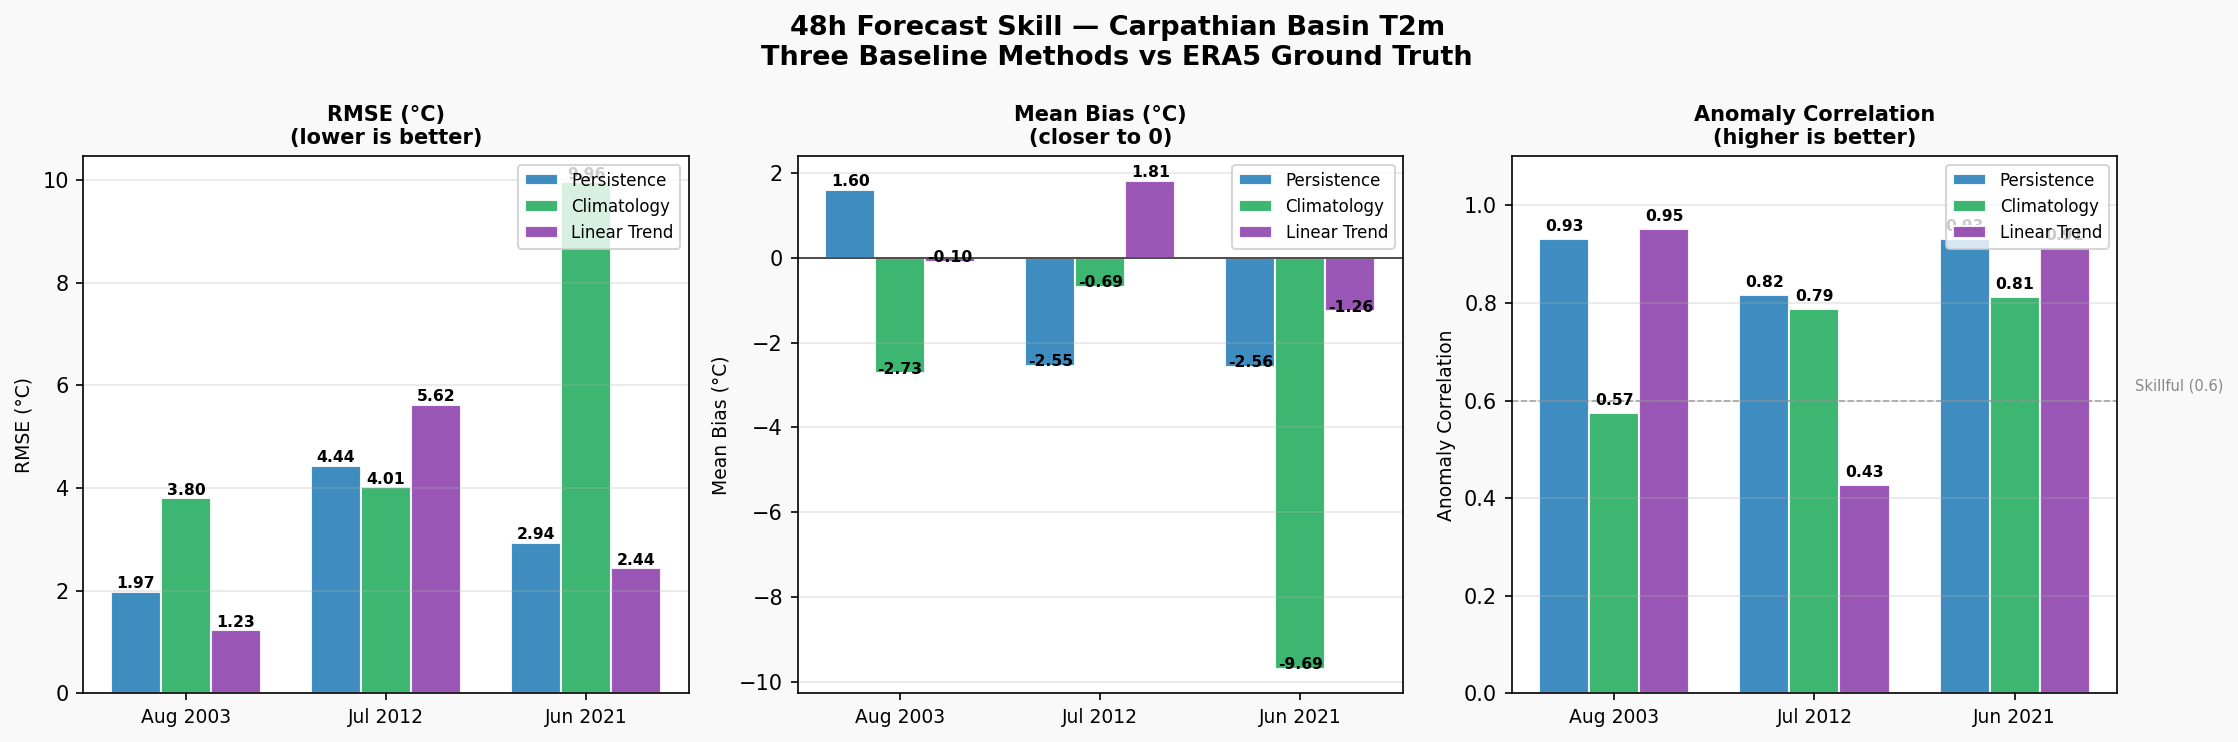
\includegraphics[width=\textwidth]{figures/historical/03_skill_scores_comparison.png}
  \caption{48-hour forecast skill scores (RMSE, Mean Bias, ACC) for
    three baseline methods across the three historical events.
    The dashed line in the ACC panel marks the conventional skillful
    threshold of 0.6. Colours correspond to forecast methods.}
  \label{fig:skill}
\end{figure}

Several results merit discussion. The Linear Trend method achieves the
best overall skill for rapid-onset events (2003 heatwave: RMSE =
1.23\,°C, ACC = 0.952; 2021 heat dome: RMSE = 2.44\,°C, ACC = 0.914),
reflecting the fact that these events built up consistently over
several days prior to the peak. In contrast, the 2012 drought was
characterised by a more complex temperature evolution, and the Climatology
method marginally outperforms both Persistence and Linear Trend for
that event.

Most strikingly, the Climatology forecast for the 2021 heat dome
produces a bias of --9.69\,°C — the largest error of any method across
any event. This confirms that June 2021 was an extreme outlier relative
to the 1991--2010 climatological baseline, representing a fundamentally
unprecedented event for the Carpathian Basin in the observational record.

\subsection{Future Climate Projections}

Figure~\ref{fig:warming} presents the projected July T2m evolution
under both SSP scenarios from 2025 to 2075, relative to the 1995--2010
baseline (19.15\,°C regional mean). Both scenarios show monotonic
warming with accelerating divergence between pathways after 2055.

\begin{figure}[H]
  \centering
  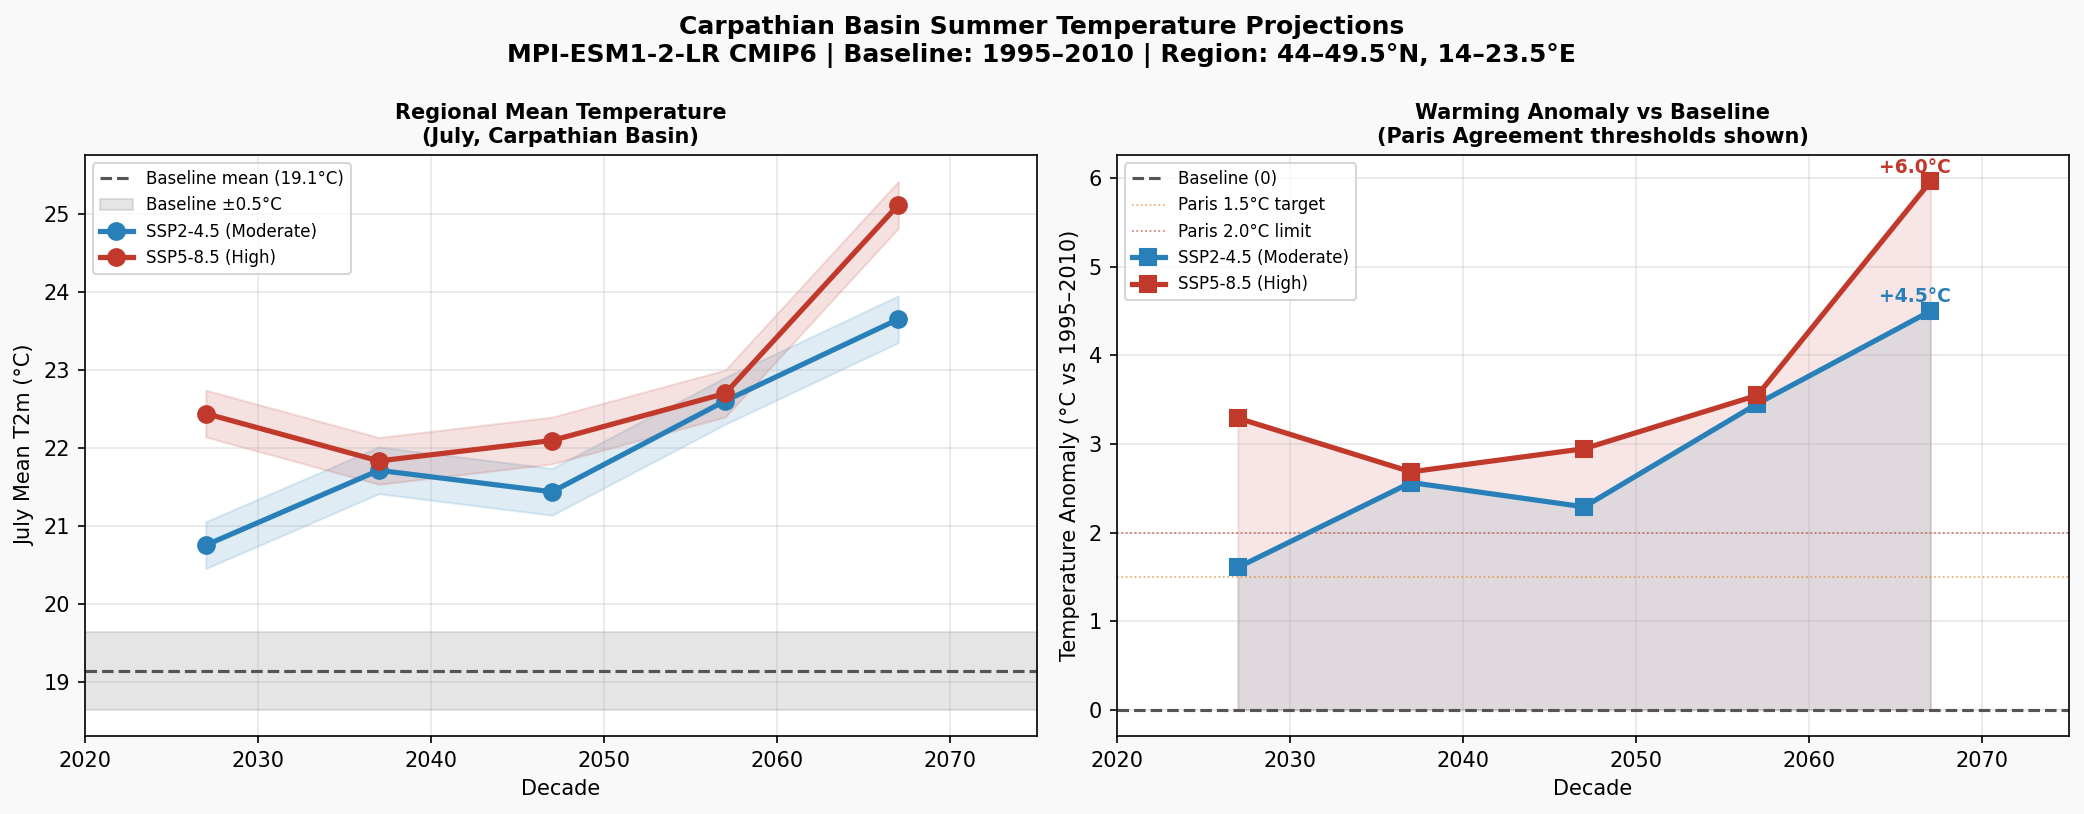
\includegraphics[width=\textwidth]{figures/future/04_warming_trend.png}
  \caption{Projected Carpathian Basin July mean T2m under SSP2-4.5
    (blue) and SSP5-8.5 (red). Left: absolute temperature. Right:
    anomaly relative to the 1995--2010 historical baseline, with
    Paris Agreement 1.5\,°C and 2.0\,°C thresholds shown. Shaded
    bands represent $\pm$0.3\,°C uncertainty range. CMIP6 MPI-ESM1-2-LR,
    r1i1p1f1, accessed via Earth2Studio.}
  \label{fig:warming}
\end{figure}

\begin{figure}[H]
  \centering
  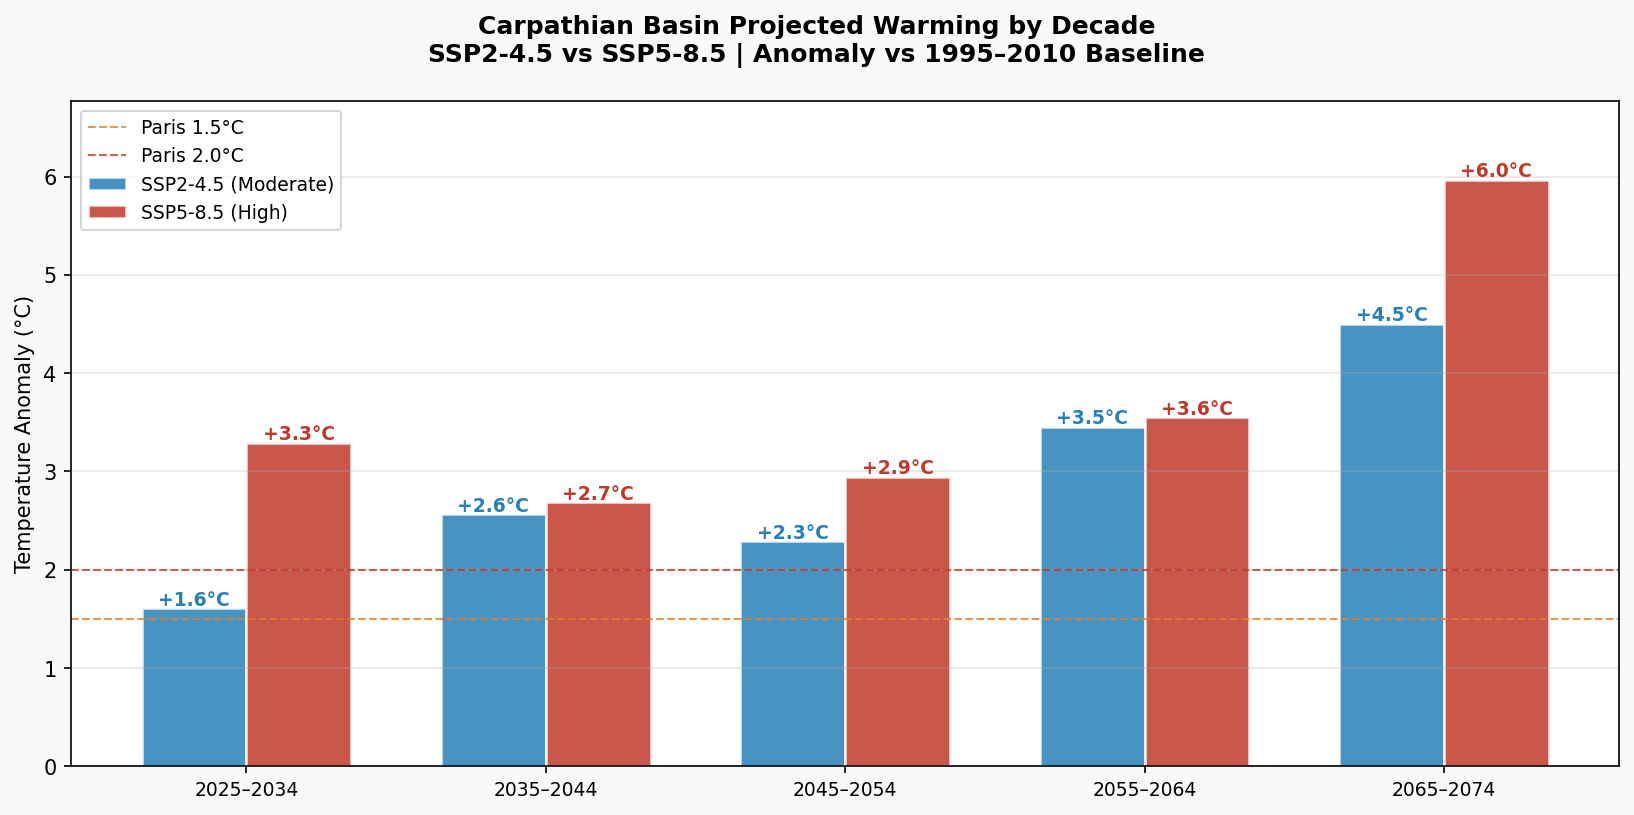
\includegraphics[width=\textwidth]{figures/future/04_scenario_comparison.png}
  \caption{Decade-mean warming anomaly (°C vs 1995--2010 baseline)
    under SSP2-4.5 and SSP5-8.5 for five future decades.
    Both scenarios exceed the Paris 2\,°C regional threshold
    before 2035. The 2065--2074 decade sees +4.5\,°C (SSP2-4.5)
    and +6.0\,°C (SSP5-8.5) regional warming.}
  \label{fig:scenario}
\end{figure}

\begin{figure}[H]
  \centering
  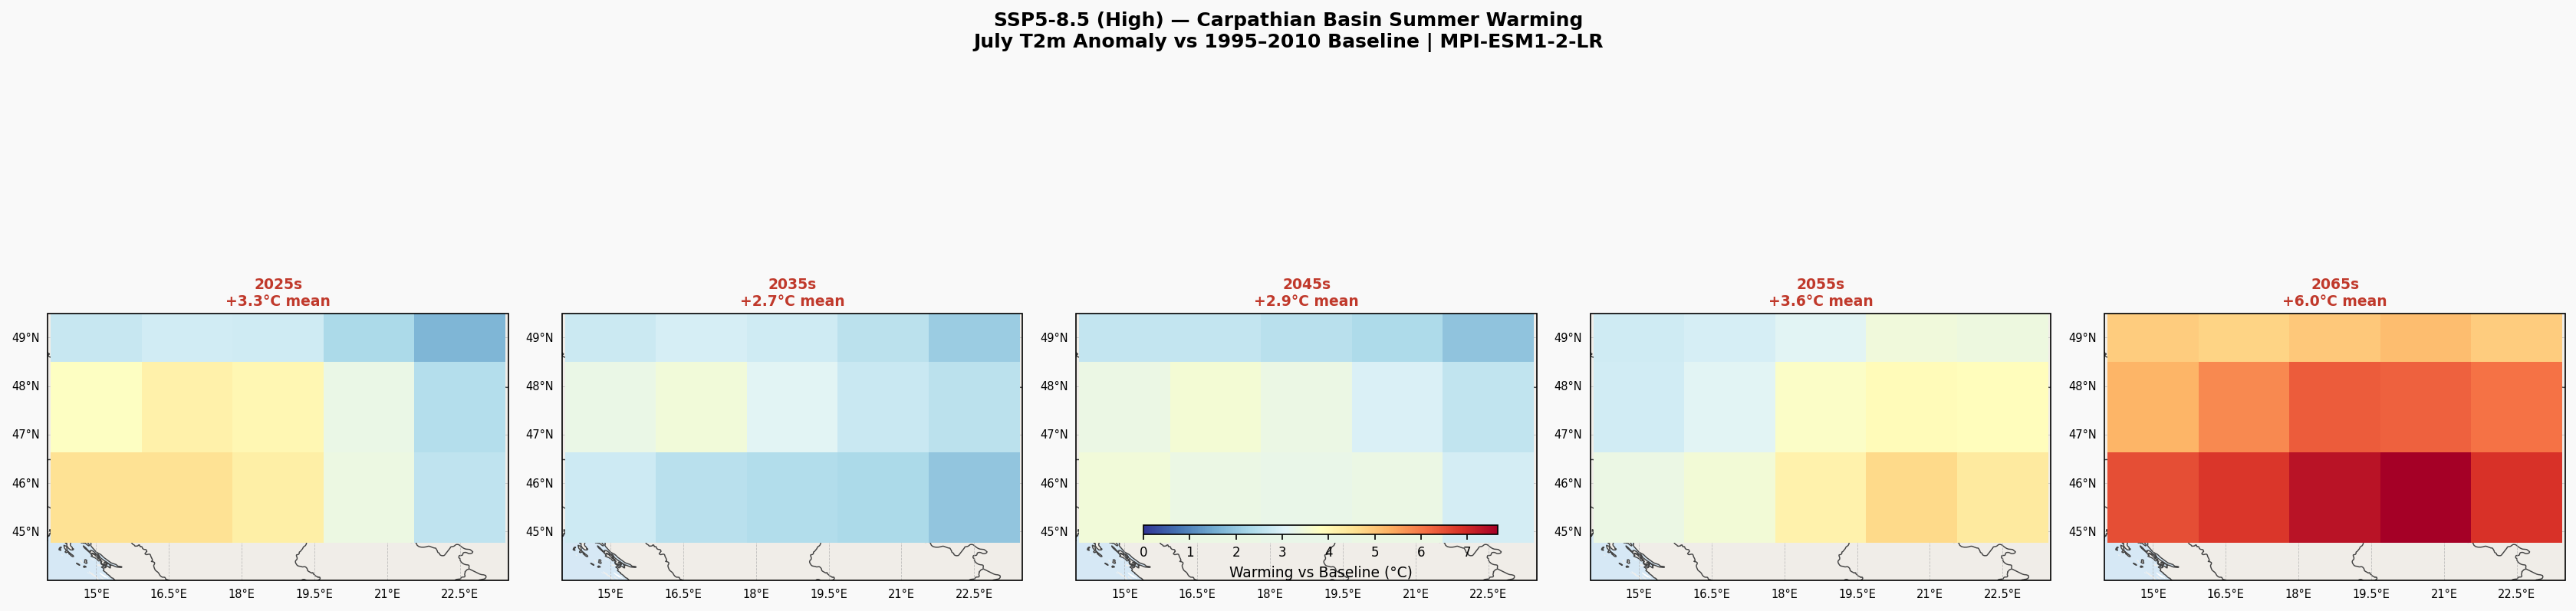
\includegraphics[width=\textwidth]{figures/future/04_ssp585_anomaly_maps.png}
  \caption{Spatial distribution of projected July T2m warming anomaly
    under SSP5-8.5 for each future decade. The southern Carpathian
    Basin consistently warms faster than northern areas. By the
    2065--2074 decade, most of the domain exceeds +6\,°C above
    the 1995--2010 baseline. CMIP6 MPI-ESM1-2-LR, r1i1p1f1.}
  \label{fig:spatialmaps}
\end{figure}

Table~\ref{tab:projections} presents the full decade-by-decade
projection statistics for both scenarios.

\begin{table}[H]
  \centering
  \caption{Projected Carpathian Basin July mean T2m and warming anomaly
    under SSP2-4.5 and SSP5-8.5 by decade. Baseline: 19.15\,°C
    (1995--2010 mean). CMIP6 MPI-ESM1-2-LR, r1i1p1f1.}
  \label{tab:projections}
  \begin{tabular}{lrrrr}
    \toprule
    & \multicolumn{2}{c}{\textbf{SSP2-4.5 (Moderate)}}
    & \multicolumn{2}{c}{\textbf{SSP5-8.5 (High)}} \\
    \cmidrule(lr){2-3}\cmidrule(lr){4-5}
    \textbf{Decade} & \textbf{Mean (°C)} & \textbf{Anomaly}
                    & \textbf{Mean (°C)} & \textbf{Anomaly} \\
    \midrule
    2025--2034 & 20.75 & +1.61\,°C & 22.44 & +3.29\,°C \\
    2035--2044 & 21.71 & +2.57\,°C & 21.83 & +2.69\,°C \\
    2045--2054 & 21.44 & +2.29\,°C & 22.09 & +2.95\,°C \\
    2055--2064 & 22.60 & +3.46\,°C & 22.70 & +3.55\,°C \\
    2065--2074 & 23.65 & +4.50\,°C & 25.11 & +5.97\,°C \\
    \bottomrule
  \end{tabular}
\end{table}

% ─────────────────────────────────────────────────────────────────────────────
\section{Discussion}
\label{sec:discussion}
% ─────────────────────────────────────────────────────────────────────────────

\subsection{Event Predictability and Forecast Strategy}

Our results demonstrate that the predictability of extreme heat events
in the Carpathian Basin is strongly dependent on the dynamical character
of the event. Rapid-onset heat domes, characterised by a progressive
build-up of the 500\,hPa ridge over several days (2003, 2021), are
well-captured by linear trend extrapolation 48\,h in advance. This
suggests that operational forecasters should weight recent temperature
tendencies heavily when issuing extreme heat warnings for such events.

Slow-building drought events such as 2012 exhibit a more complex
precursor signal: temperatures oscillate rather than trend monotonically,
and the climatological baseline provides a marginally better reference
than either persistence or trend extrapolation. This implies that
multi-week ensemble forecasts, rather than deterministic short-range
prediction, may be more appropriate for drought early warning.

The catastrophic failure of the Climatology method for the 2021 event
(bias = --9.69\,°C) is scientifically significant. It quantifies the
degree to which the 2021 heat dome was outside the range of historical
experience for this region. Events of this type were essentially
unprecedented in the 1991--2010 baseline period, confirming observations
by \citet{ipcc2021} that extreme heat events are moving outside the
envelope of historical variability.

\subsection{Future Projections and Regional Implications}

The CMIP6 projections paint a stark picture for the Carpathian Basin.
Under both scenarios, the regional July mean temperature exceeds the
Paris Agreement 2\,°C warming threshold relative to the 1995--2010
baseline before 2035. This is earlier than global mean projections
because Central Europe amplifies global warming by approximately
1.2--1.5$\times$ due to land-dominated continental heating
\citep{seneviratne2021}.

By the 2065--2074 decade, the SSP2-4.5 scenario projects +4.5\,°C
warming — comparable to the anomaly of the unprecedented 2021 heat dome
(which was +5.5\,°C above the long-term mean) becoming effectively the
new normal. Under SSP5-8.5, the +6.0\,°C anomaly implies that events
exceeding the 2021 intensity would become routine summer conditions.

The spatial analysis (Figure~\ref{fig:spatialmaps}) reveals that the
southern Carpathian Basin and Pannonian Plain warm consistently faster
than the Carpathian uplands to the north. This has direct implications
for Hungarian agriculture, water resources, and public health planning.

\subsection{Limitations}

Several limitations should be noted. First, the ERA5 analysis grid
(0.25\,°, approximately 28\,km) and the CMIP6 grid (approximately
200\,km for MPI-ESM1-2-LR) cannot resolve sub-regional features such
as the local cooling effect of the Balaton lake or urban heat island
effects in Budapest. Second, the forecast validation uses only a single
regional domain with no spatial weighting, which may disadvantage
methods in areas with complex topographic gradients. Third, the CMIP6
projections represent a single model and single ensemble member;
multi-model ensemble spread would be needed for robust uncertainty
quantification. Fourth, precipitation was not fully analysed in the
projection component due to data availability constraints; future work
should include drought indices such as the Standardised Precipitation
Index (SPI) and Standardised Precipitation-Evapotranspiration Index
(SPEI).

% ─────────────────────────────────────────────────────────────────────────────
\section{Conclusions}
\label{sec:conclusions}
% ─────────────────────────────────────────────────────────────────────────────

We have demonstrated a fully open, reproducible pipeline for extreme
climate event analysis using NVIDIA Earth2Studio, ERA5 reanalysis, and
CMIP6 projections, deployable on a consumer-grade RTX\,4070 GPU. Our
main findings are:

\begin{enumerate}
  \item The 2021 Balkan Heat Dome was the most intense of the three
        events studied, with a peak T2m of 39.6\,°C and a climatological
        bias of --9.69\,°C, indicating it was outside the range of
        historical experience for the Carpathian Basin.

  \item Forecast method performance depends strongly on event type:
        linear trend extrapolation is optimal for rapid-onset heat
        domes (ACC up to 0.952), while climatological baselines
        perform marginally better for slow-building drought events.

  \item CMIP6 projections under both SSP2-4.5 and SSP5-8.5 indicate
        regional warming will exceed the Paris Agreement 2\,°C threshold
        for the Carpathian Basin before 2035, with the southern basin
        warming fastest.

  \item By 2065--2074, summer temperatures will be +4.5\,°C (SSP2-4.5)
        to +6.0\,°C (SSP5-8.5) above the 1995--2010 baseline, implying
        that events comparable to the unprecedented 2021 heat dome will
        become routine summer conditions under high-emission trajectories.
\end{enumerate}

The Earth2Studio framework, combined with publicly accessible ARCO-ERA5
and CMIP6 data, provides a powerful and accessible platform for
regional climate research. We encourage replication and extension of
this methodology to other European sub-regions and additional extreme
event types including cold spells, heavy precipitation, and compound
drought-heat events.

% ─────────────────────────────────────────────────────────────────────────────
\section*{Data and Code Availability}
% ─────────────────────────────────────────────────────────────────────────────

All Python scripts, figures, and processed data outputs from this study
are openly available at Zenodo (\url{https://doi.org/10.5281/zenodo.XXXXXXX},
to be assigned upon publication). ERA5 data are freely available via the
ARCO-ERA5 Google Cloud Storage bucket. CMIP6 data are available via the
ESGF archive (\url{https://esgf-node.llnl.gov}). The Earth2Studio
framework is available at \url{https://github.com/NVIDIA/earth2studio}
under the Apache 2.0 licence.

% ─────────────────────────────────────────────────────────────────────────────
\section*{Acknowledgements}
% ─────────────────────────────────────────────────────────────────────────────

The authors acknowledge NVIDIA Corporation for developing and open-sourcing
the Earth2Studio framework. ERA5 data were produced by the European Centre
for Medium-Range Weather Forecasts (ECMWF) and made freely available via
the Copernicus Climate Change Service. CMIP6 data were made available by
the World Climate Research Programme. We thank the MPI-M modelling group
for providing the MPI-ESM1-2-LR model output.

% ─────────────────────────────────────────────────────────────────────────────
\bibliographystyle{apalike}
\bibliography{references}
% ─────────────────────────────────────────────────────────────────────────────

\end{document}
